\documentclass[t,xcolor={dvipsnames},final,aspectratio=169]{beamer}
\beamertemplatenavigationsymbolsempty
\usepackage{adjustbox}
\usepackage{graphicx}
\usepackage{amsmath}
\usepackage{amsfonts}
\usepackage{url}
\usepackage{hyperref}
\usepackage{tikz}
\usepackage{smartdiagram}
\usepackage{booktabs}

\newcommand{\kp}{Clinical Psychology}

\mode<presentation> {
    \usetheme{Frankfurt}
    \usecolortheme{crane}
    \setbeamertemplate{footline}[frame number]
    \beamerdefaultoverlayspecification{<+->}
}

\title{How to handle LLMs in your research}
\author{Pablo Mosteiro, Robert Bagheri\\
\tiny{Partly generated with help of Qwen/Qwen2.5-7B-Instruct and moonshotai/Kimi-K2-Instruct-0905 via together and groq, respectively (HuggingChat).}}
\institute{Department of Methodology \& Statistics}
\date{\today}
\logo{
\includegraphics[scale=0.5]{img/UU-logo2011_CMYK-eps-converted-to.pdf}\hspace*{0.65\textwidth}\vspace{-8mm}}

\begin{document}

\begin{frame}
    \maketitle
\end{frame}

\begin{frame}{Today's Agenda}
    \begin{itemize}
        \item Introduction (5 min)
        \item AI, ML, and LLMs (5 min)
        \item How LLMs Work (5 min)
        \item Limitations and Risks (10 min)
        \item Practical LLM Use in Research (10 min)
        \item Prompting CAs and Chatbots (10 min)
        \item Conclusion (5 min)
    \end{itemize}
\end{frame}

\section{Intro}

{\setbeamertemplate{logo}{}
{
\begin{frame}{About us}
\begin{center}
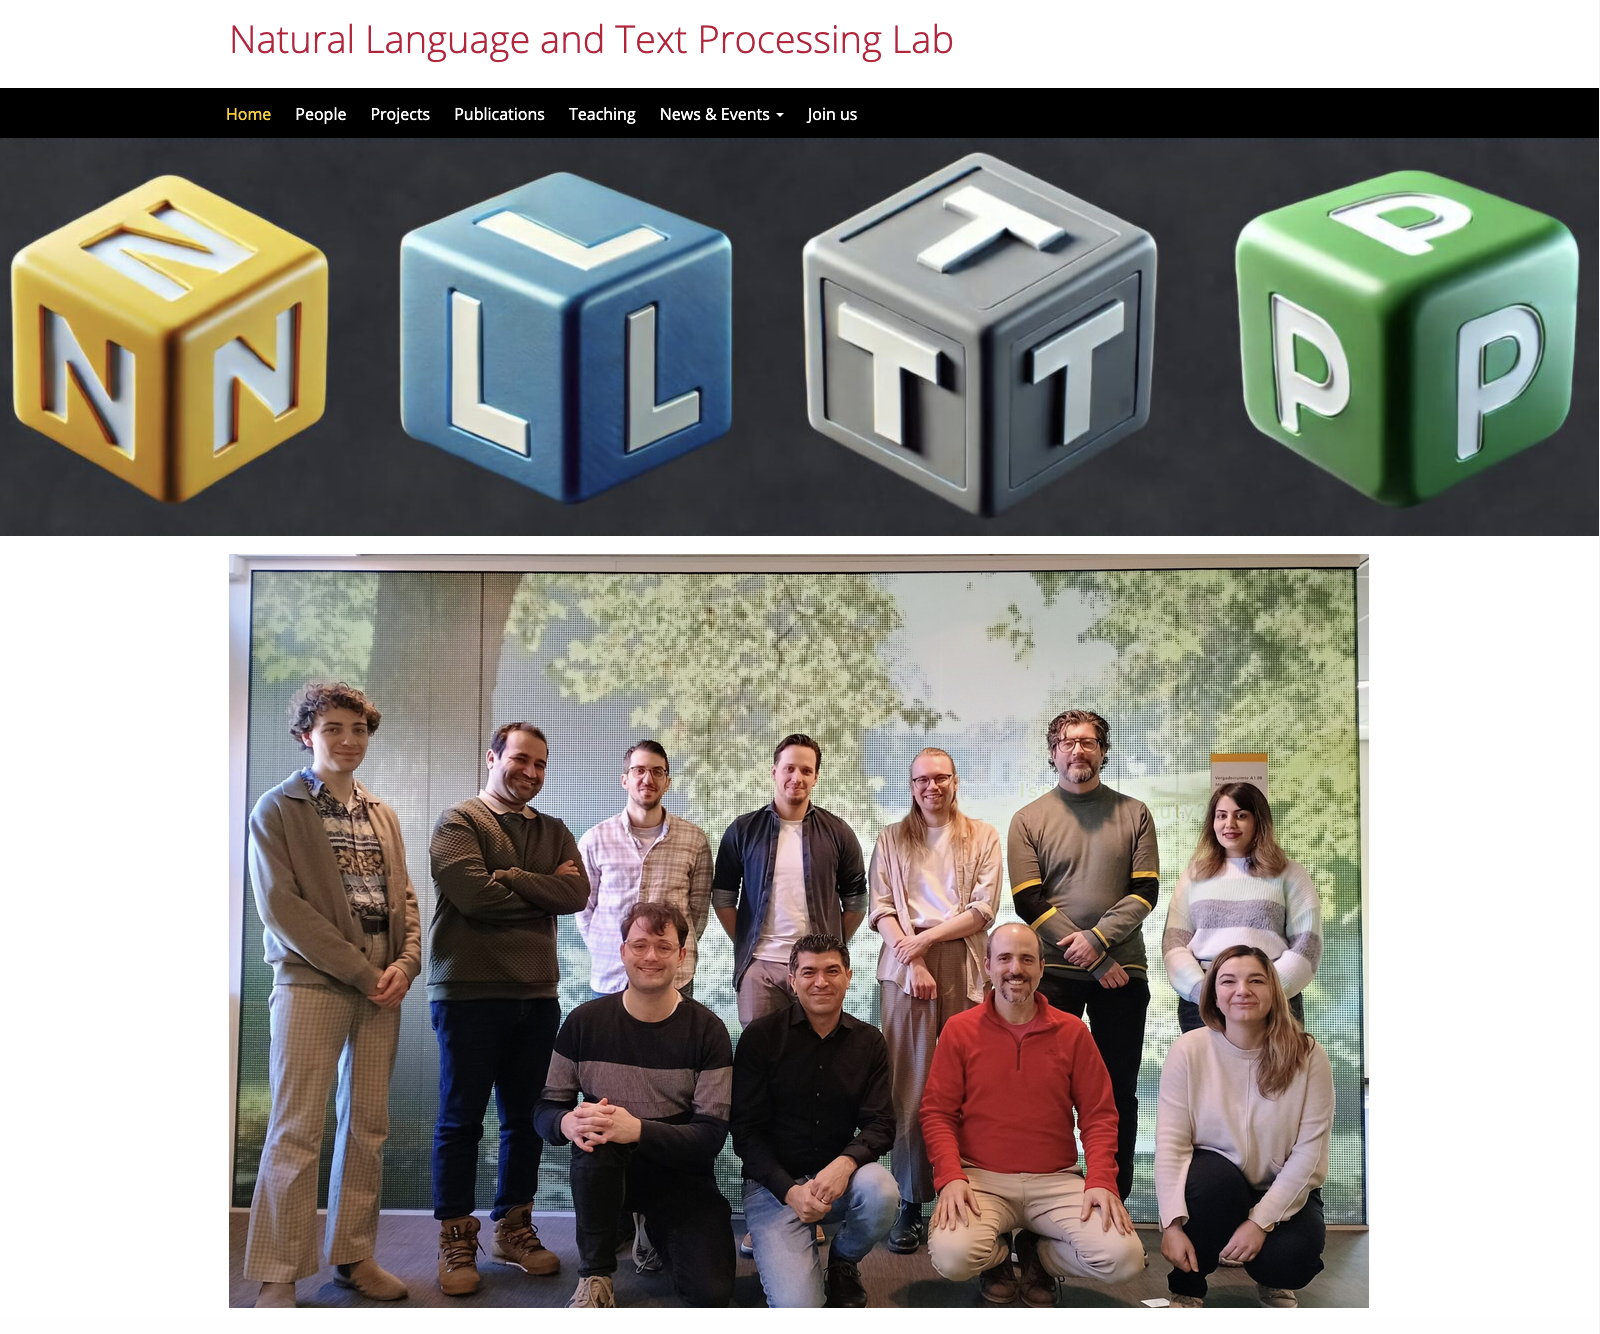
\includegraphics[width=0.5\textwidth]{img/nltp.png}

\url{https://nlp.sites.uu.nl/}
\end{center}
\end{frame}
}

\begin{frame}{Introduction: What do you know about LLMs?}
\begin{itemize}
\item    \textbf{Activity: Think-Pair-Share} (2 min)
    \end{itemize}
\end{frame}

\section{AI, ML, LLMs}
\begin{frame}{Artificial Intelligence, ML, and LLMs: Key Definitions}
    \textbf{Artificial Intelligence (AI)}
    \begin{itemize}
        \item Computer systems performing tasks requiring human intelligence
        \item Examples: Chess playing, image recognition, language translation
    \end{itemize}
    
    \textbf{Machine Learning (ML)}
    \begin{itemize}
        \item Subset of AI using algorithms that improve through experience
        \item Learns patterns from data without explicit programming
    \end{itemize}
    
    \textbf{Large Language Models (LLMs)}
    \begin{itemize}
        \item AI systems trained on vast text amounts
        \item Understand and generate human language
        \item Examples: GPT, Claude, Qwen, Mistral
    \end{itemize}
\end{frame}

\begin{frame}{AI vs ML vs LLM: The Relationship}
    \begin{center}
    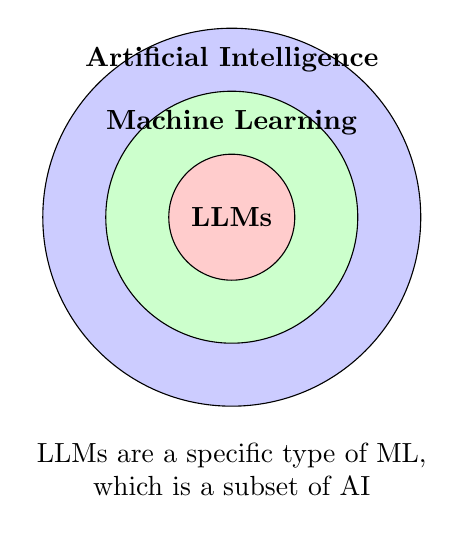
\begin{tikzpicture}[scale=0.8]
        \draw[fill=blue!20] (0,0) circle (3cm);
        \node at (0,2.5) {\textbf{Artificial Intelligence}};
        
        \draw[fill=green!20] (0,0) circle (2cm);
        \node at (0,1.5) {\textbf{Machine Learning}};
        
        \draw[fill=red!20] (0,0) circle (1cm);
        \node at (0,0) {\textbf{LLMs}};
        
        \node[align=center] at (0,-4) {LLMs are a specific type of ML,\\ which is a subset of AI};
    \end{tikzpicture}
    \end{center}
\end{frame}

\section{How LLMs work}
\begin{frame}{Model Learning Process: Training Phase}
    \textbf{Training Phase}
    \begin{itemize}
        \item Model learns patterns from large datasets
        \item Adjusts internal parameters to minimize prediction errors
        \item Requires massive computational resources
        \item Can take weeks or months for large models
    \end{itemize}
    
    \textbf{Example}: LLM learns that "cat" often appears with "dog" in pet-related contexts
\end{frame}

\begin{frame}{Model Learning Process: Validation Phase}
    \textbf{Validation Phase}
    \begin{itemize}
        \item Test model on new, unseen data
        \item Measure performance using metrics (accuracy, precision, recall)
        \item Prevent overfitting (memorizing training data)
        \item Tune hyperparameters for optimal performance
    \end{itemize}
    
    \textbf{Key insight}: Good models generalize to new data, not just memorize training examples
\end{frame}

\begin{frame}{Model Learning Process: Biases}
    \textbf{Common Biases in LLMs}
    \begin{itemize}
        \item \textbf{Training data bias:} Reflects biases in source material
        \item \textbf{Representation bias:} Underrepresents certain groups
        \item \textbf{Confirmation bias:} Reinforces existing beliefs
        \item \textbf{Temporal bias:} Becomes outdated as language/society changes
    \end{itemize}
    
    \textbf{Real-world impact}: Biased models can perpetuate harmful stereotypes
\end{frame}

\begin{frame}{What is Generative AI?}
    \textbf{Definition}: AI that creates new content (text, images, code, audio)
    
    \textbf{Key Features}:
    \begin{itemize}
        \item Creates novel outputs, not just classifies
        \item Learns patterns from training data
        \item Generates human-like content
    \end{itemize}
    
    \textbf{Examples}: ChatGPT (text), DALL-E (images), CodeT5 (code)
\end{frame}

\begin{frame}{Generative AI vs. Other Models}
    \begin{center}
    \begin{tabular}{lcc}
    \toprule
    \textbf{Feature} & \textbf{Generative} & \textbf{Discriminative} \\
    \midrule
    Primary Task & Create new content & Classify existing data \\
    Output Type & Novel text/images & Labels/categories \\
    Learning Focus & Data distribution & Decision boundaries \\
    Example & GPT, DALL-E & Spam filters, medical diagnosis \\
    \bottomrule
    \end{tabular}
    \end{center}
\end{frame}

\begin{frame}{Activity: True or False?}
    \textbf{Instructions}: Raise your hand if you think the statement is TRUE
    
    \textbf{Statement 1}: Generative AI can only work with text
    
    \textbf{Statement 2}: All generative models are also discriminative
    
    \textbf{Statement 3}: Generative AI creates completely original content never seen in training
    
    \textbf{Statement 4}: LLMs are a type of generative AI
\end{frame}

\section{Limitations and Risks}
\begin{frame}{Limitations and Risks: Hallucinations}
    \textbf{What are hallucinations?}
    \begin{itemize}
        \item LLMs generate false or nonsensical information
        \item Appears confident and plausible
        \item Can include fake citations, non-existent facts
    \end{itemize}
    
    \textbf{Example}: Asking for "recent studies on X" might return made-up citations
    
    \textbf{Risk}: Researchers might unknowingly use false information
\end{frame}

\begin{frame}{Limitations and Risks: Bias}
    \textbf{Types of Bias}
    \begin{itemize}
        \item \textbf{Gender bias:} Assumes doctors are male, nurses are female
        \item \textbf{Racial bias:} Associates certain groups with negative stereotypes
        \item \textbf{Cultural bias:} Primarily represents Western perspectives
        \item \textbf{Academic bias:} Favors published, English-language sources
    \end{itemize}
    
    \textbf{Activity}: Can you identify bias in this LLM output?
\end{frame}

\begin{frame}{Limitations and Risks: Output Reliability}
    \textbf{Reliability Issues}
    \begin{itemize}
        \item \textbf{Inconsistency:} Same prompt can yield different answers
        \item \textbf{Context dependency:} Performance varies by domain
        \item \textbf{Temporal drift:} Knowledge becomes outdated
        \item \textbf{Prompt sensitivity:} Small changes affect outputs significantly
    \end{itemize}
    
    \textbf{Best practice}: Always verify critical information from multiple sources
\end{frame}

\begin{frame}{Limitations and Risks: Ethics}
    \textbf{Ethical Concerns}
    \begin{itemize}
        \item \textbf{Data:} Training data may include personal or copyrighted material
        \item \textbf{Environmental impact:} High energy consumption
        \item \textbf{Labor practices:} Data annotation often involves poor working conditions
        \only<3>{\hfill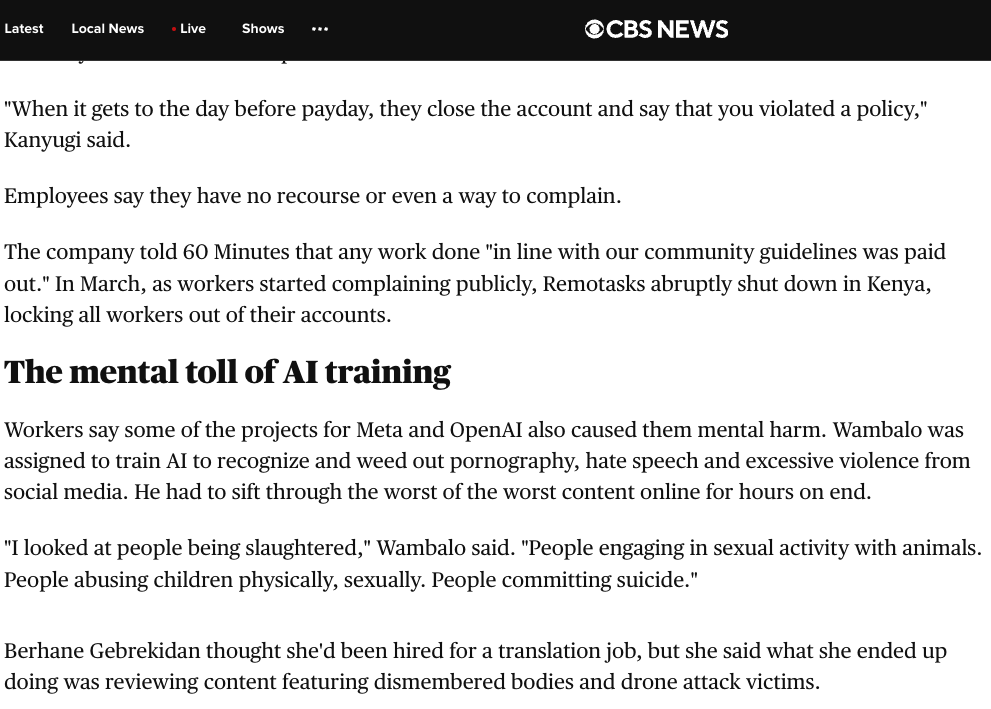
\includegraphics[height=4cm]{img/labor.png}\\
        \footnotesize{\url{https://www.cbsnews.com/news/ai-work-kenya-exploitation-60-minutes} (Nov 2024)}
}  % visible only on slide 4
        \item \textbf{Academic integrity:} attribution of AI assistance / uploading restricted data
        \item \textbf{Open source:} Often little documentation on data, training, architecture\\
        \only<5>{``Given both the competitive landscape and the safety implications of large-scale models like GPT-4, this report contains no further details about the architecture (including model size), hardware, training compute, dataset construction, training method, or similar''

OpenAI: Achiam, J. et al (2024). \textit{GPT-4 Technical Report}. \url{https://arxiv.org/abs/2303.08774}}
\item \textbf{Effect on cognition:}  
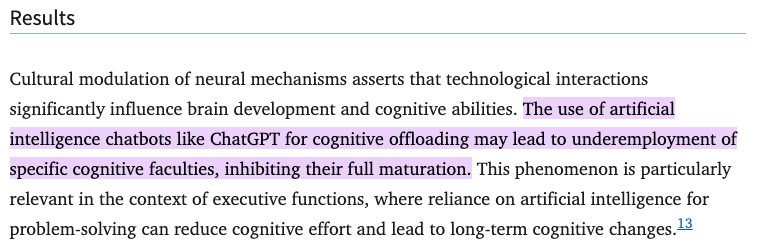
\includegraphics[width=0.6\textwidth]{img/cognition.png}\\
\footnotesize{Dubey et al. Redefining Cognitive Domains in the Era of ChatGPT: A Comprehensive Analysis of Artificial Intelligence's Influence and Future Implications. Med Res Arch. 2024 Jun;12(6):5383}
    \end{itemize}
\end{frame}

\section{Practical LLM Use in Research}

\begin{frame}{Free vs. Paid Systems}
\begin{center}

\includegraphics[width=0.9\textwidth]{img/wooclap.png}
\end{center}
\end{frame}

\begin{frame}{Free vs. Paid Systems}
    \begin{center}
    \begin{tabular}{lcc}
    \toprule
    \textbf{Feature} & \textbf{Free} & \textbf{Paid} \\
    \midrule
    Cost & €0 & €10-€100+ monthly \\
    Usage Limits & Yes & Higher/none \\
    Model Quality & Basic & Advanced \\
    Response Speed & Slower & Faster \\
    Support & Community & Professional \\
    \bottomrule
    \end{tabular}
    \end{center}
\end{frame}

\begin{frame}{Free vs. Paid: When to Choose What?}
    \textbf{Choose FREE when:}
    \begin{itemize}
        \item Learning or experimenting
        \item Occasional, non-critical use
        \item Budget constraints
        \item Simple tasks (summarization, basic Q\&A)
    \end{itemize}
    
    \textbf{Choose PAID when:}
    \begin{itemize}
        \item Professional/research work
        \item High-volume usage
        \item Need for reliability
        \item Advanced features required
    \end{itemize}
\end{frame}

\begin{frame}{LLM Use in \kp\ Research}
    \textbf{Appropriate \& Inappropriate Uses}
    \begin{itemize}
        \item Think-Pair-Share
    \end{itemize}
    \end{frame}

\begin{frame}{LLM Use in \kp\ Research: Appropriate Applications}
    \textbf{Appropriate Uses}
    \begin{itemize}
        \item \textbf{Literature review:} Summarizing papers (with verification)
        \item \textbf{Writing assistance:} Drafting, editing, proofreading
        \item \textbf{Code generation:} Writing analysis scripts
        \item \textbf{Brainstorming:} Generating research ideas
        \item \textbf{Translation:} Working with multilingual sources
    \end{itemize}
    
    \textbf{Key}: Always maintain human oversight and verification
\end{frame}

\begin{frame}{LLM Use in \kp\ Research: Inappropriate Applications}
    \textbf{Avoid Using LLMs For:}
    \begin{itemize}
        \item \textbf{Statistical analysis:} LLMs can't perform proper statistical tests
        \item \textbf{Fact-checking:} They may hallucinate information
        \item \textbf{Critical decisions:} Participant safety, ethical approvals
        \item \textbf{Original thinking:} Generating truly novel theories
        \item \textbf{Replacing expertise:} They supplement but don't replace researcher knowledge
    \end{itemize}
\end{frame}

\section{Prompting}
{\setbeamertemplate{logo}{}
{
\begin{frame}{Effective Prompting: BRAVE(R) Framework}
  \begin{columns}
    \begin{column}{0.45\textwidth}
    \begin{center}
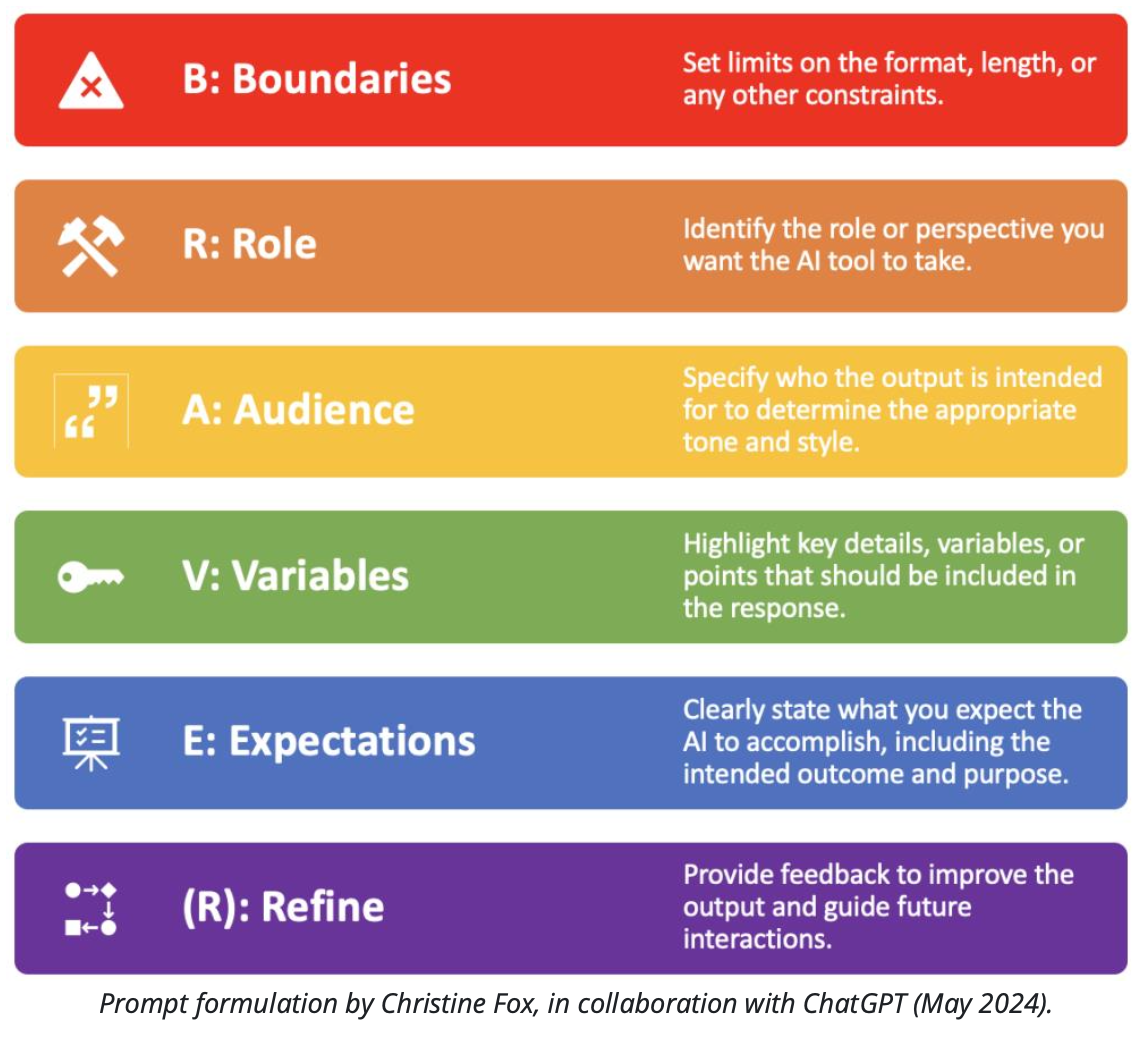
\includegraphics[width=0.9\textwidth]{img/braver.png}
\end{center}
    \end{column}
    \begin{column}{0.45\textwidth}  %%<--- here
    \textbf{Poor prompt}: ``Summarize this paper''
    
    \textbf{Better prompt}: ``Act as a psychology research assistant [R]. Summarize this paper in 3 bullet points [B] focusing on methodology and findings relevant to cognitive behavioral therapy [V]. Use academic language [A] and APA style [E].''
    
    \textbf{Key insight}: Specific, contextual prompts yield better results
    \end{column}
  \end{columns}
\end{frame}
}

\begin{frame}{Evaluating and Critically Assessing GenAI Responses}
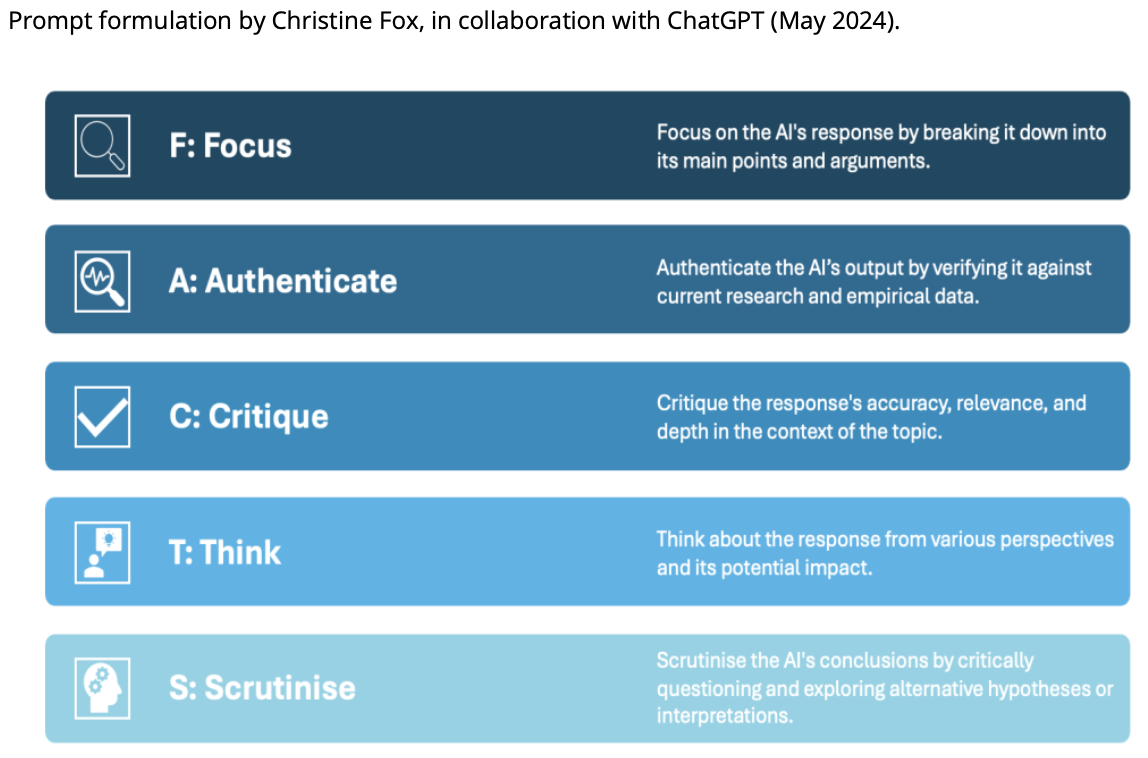
\includegraphics[width=8cm]{img/facts.png}
More info: \url{https://teachersguidegsls.nl/genai/generative-ai-guidelines/}
\end{frame}

\begin{frame}{Ways to prompt}
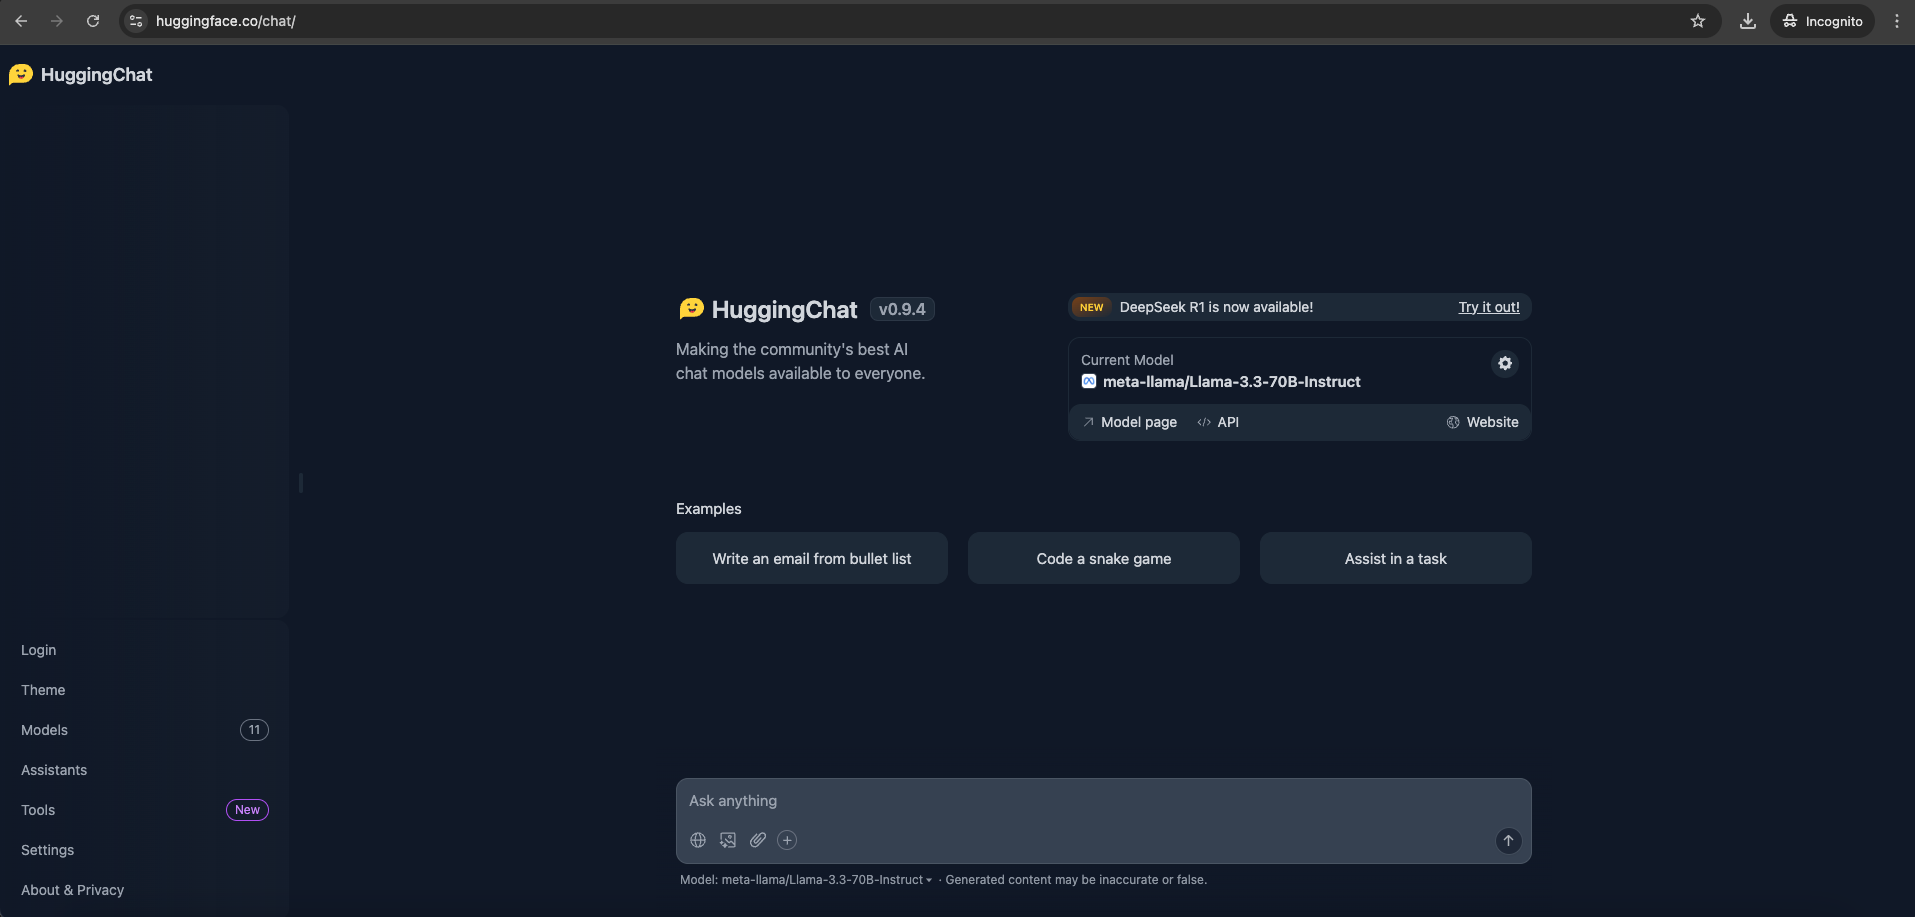
\includegraphics[width=0.9\textwidth]{img/huggingchat.png}
\end{frame}

\begin{frame}{Switch models}
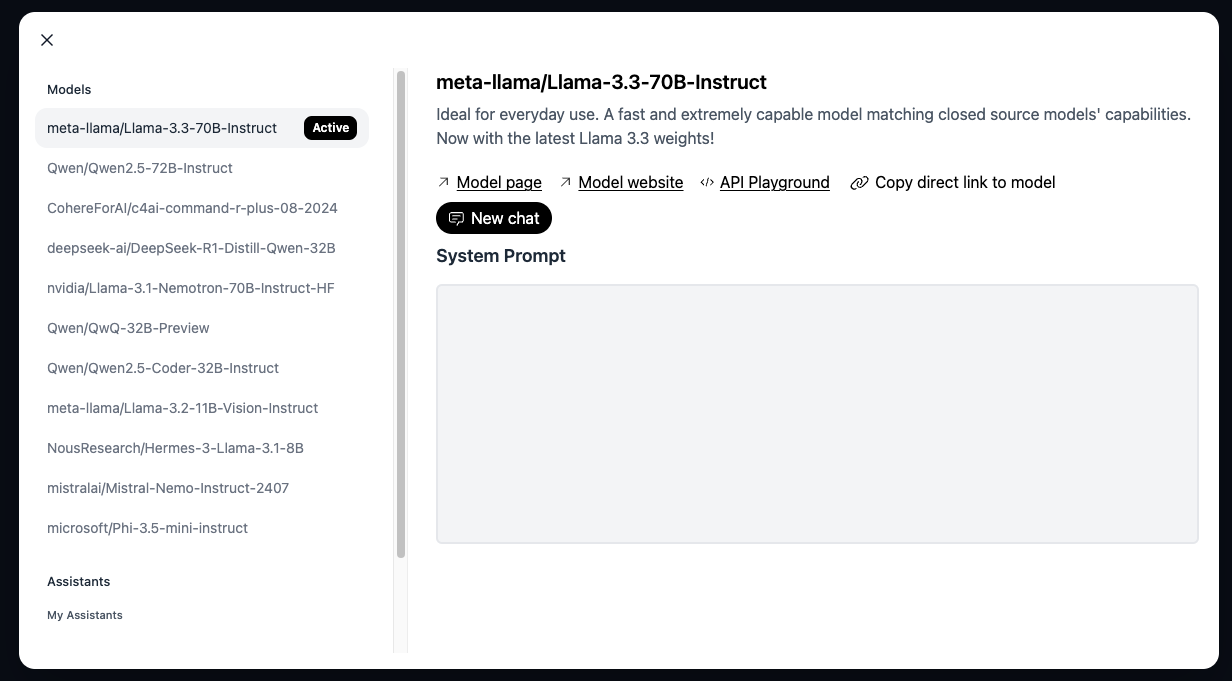
\includegraphics[width=0.9\textwidth]{img/models.png}
\end{frame}

{\setbeamertemplate{logo}{}
\begin{frame}{Using an LLM locally (no server)}
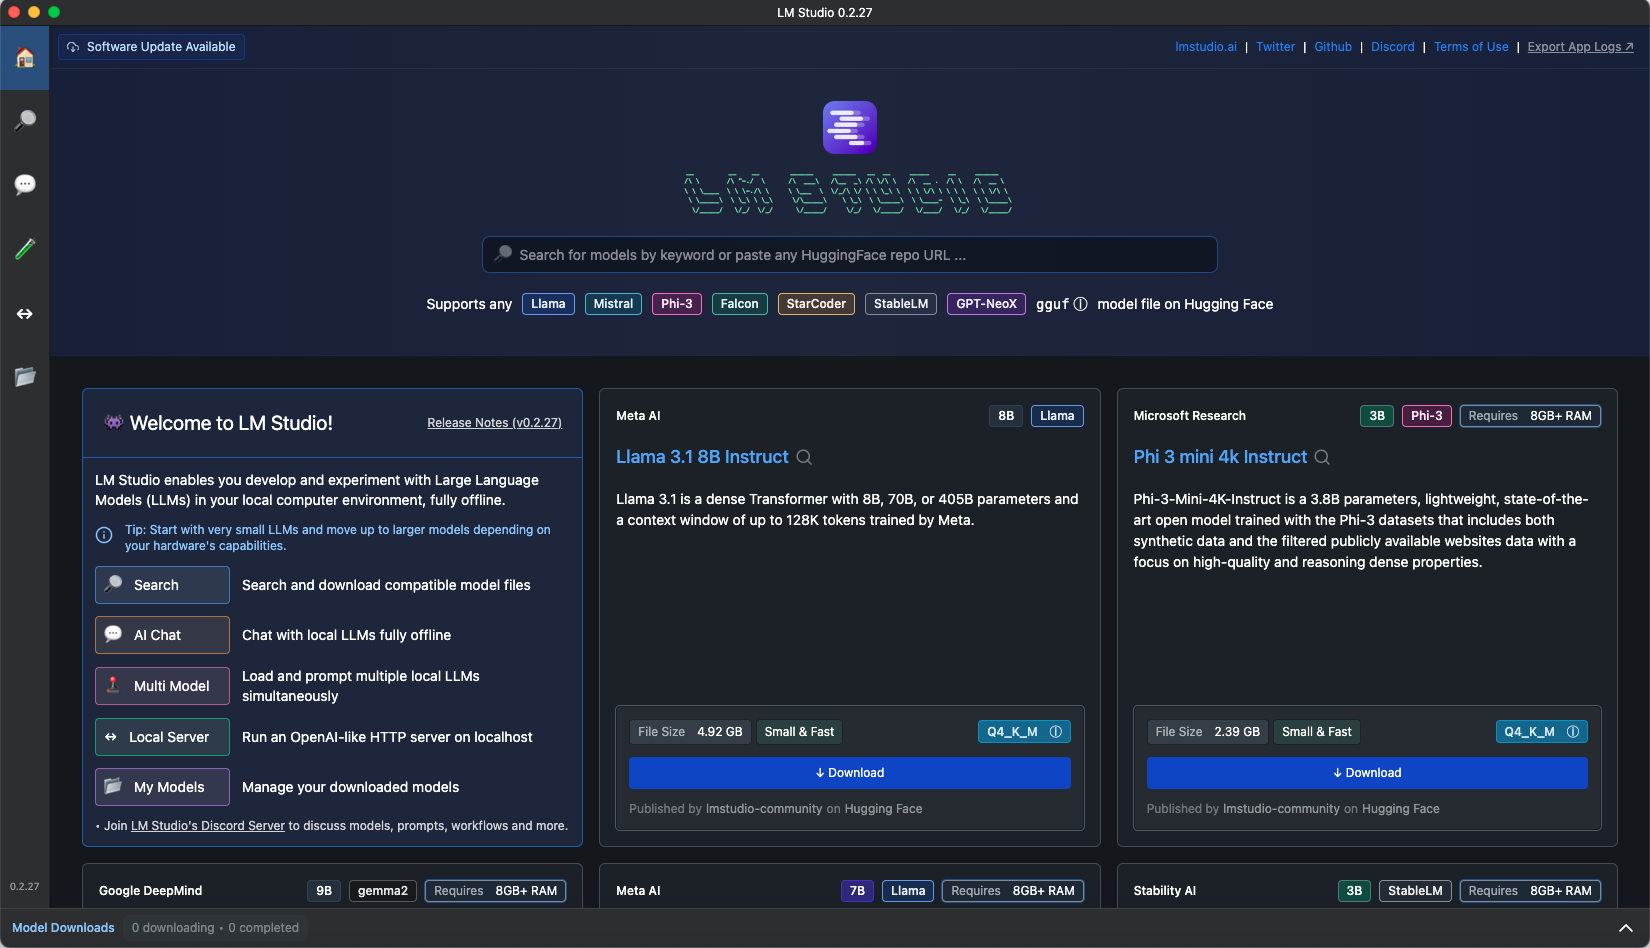
\includegraphics[width=0.8\textwidth]{img/lmstudio.png}
\note{But model can still be train in a very closed-source way}
\end{frame}
}

\begin{frame}{Versatile platform}
\begin{itemize}
\item \huge{OpenRouter.ai}
\end{itemize}
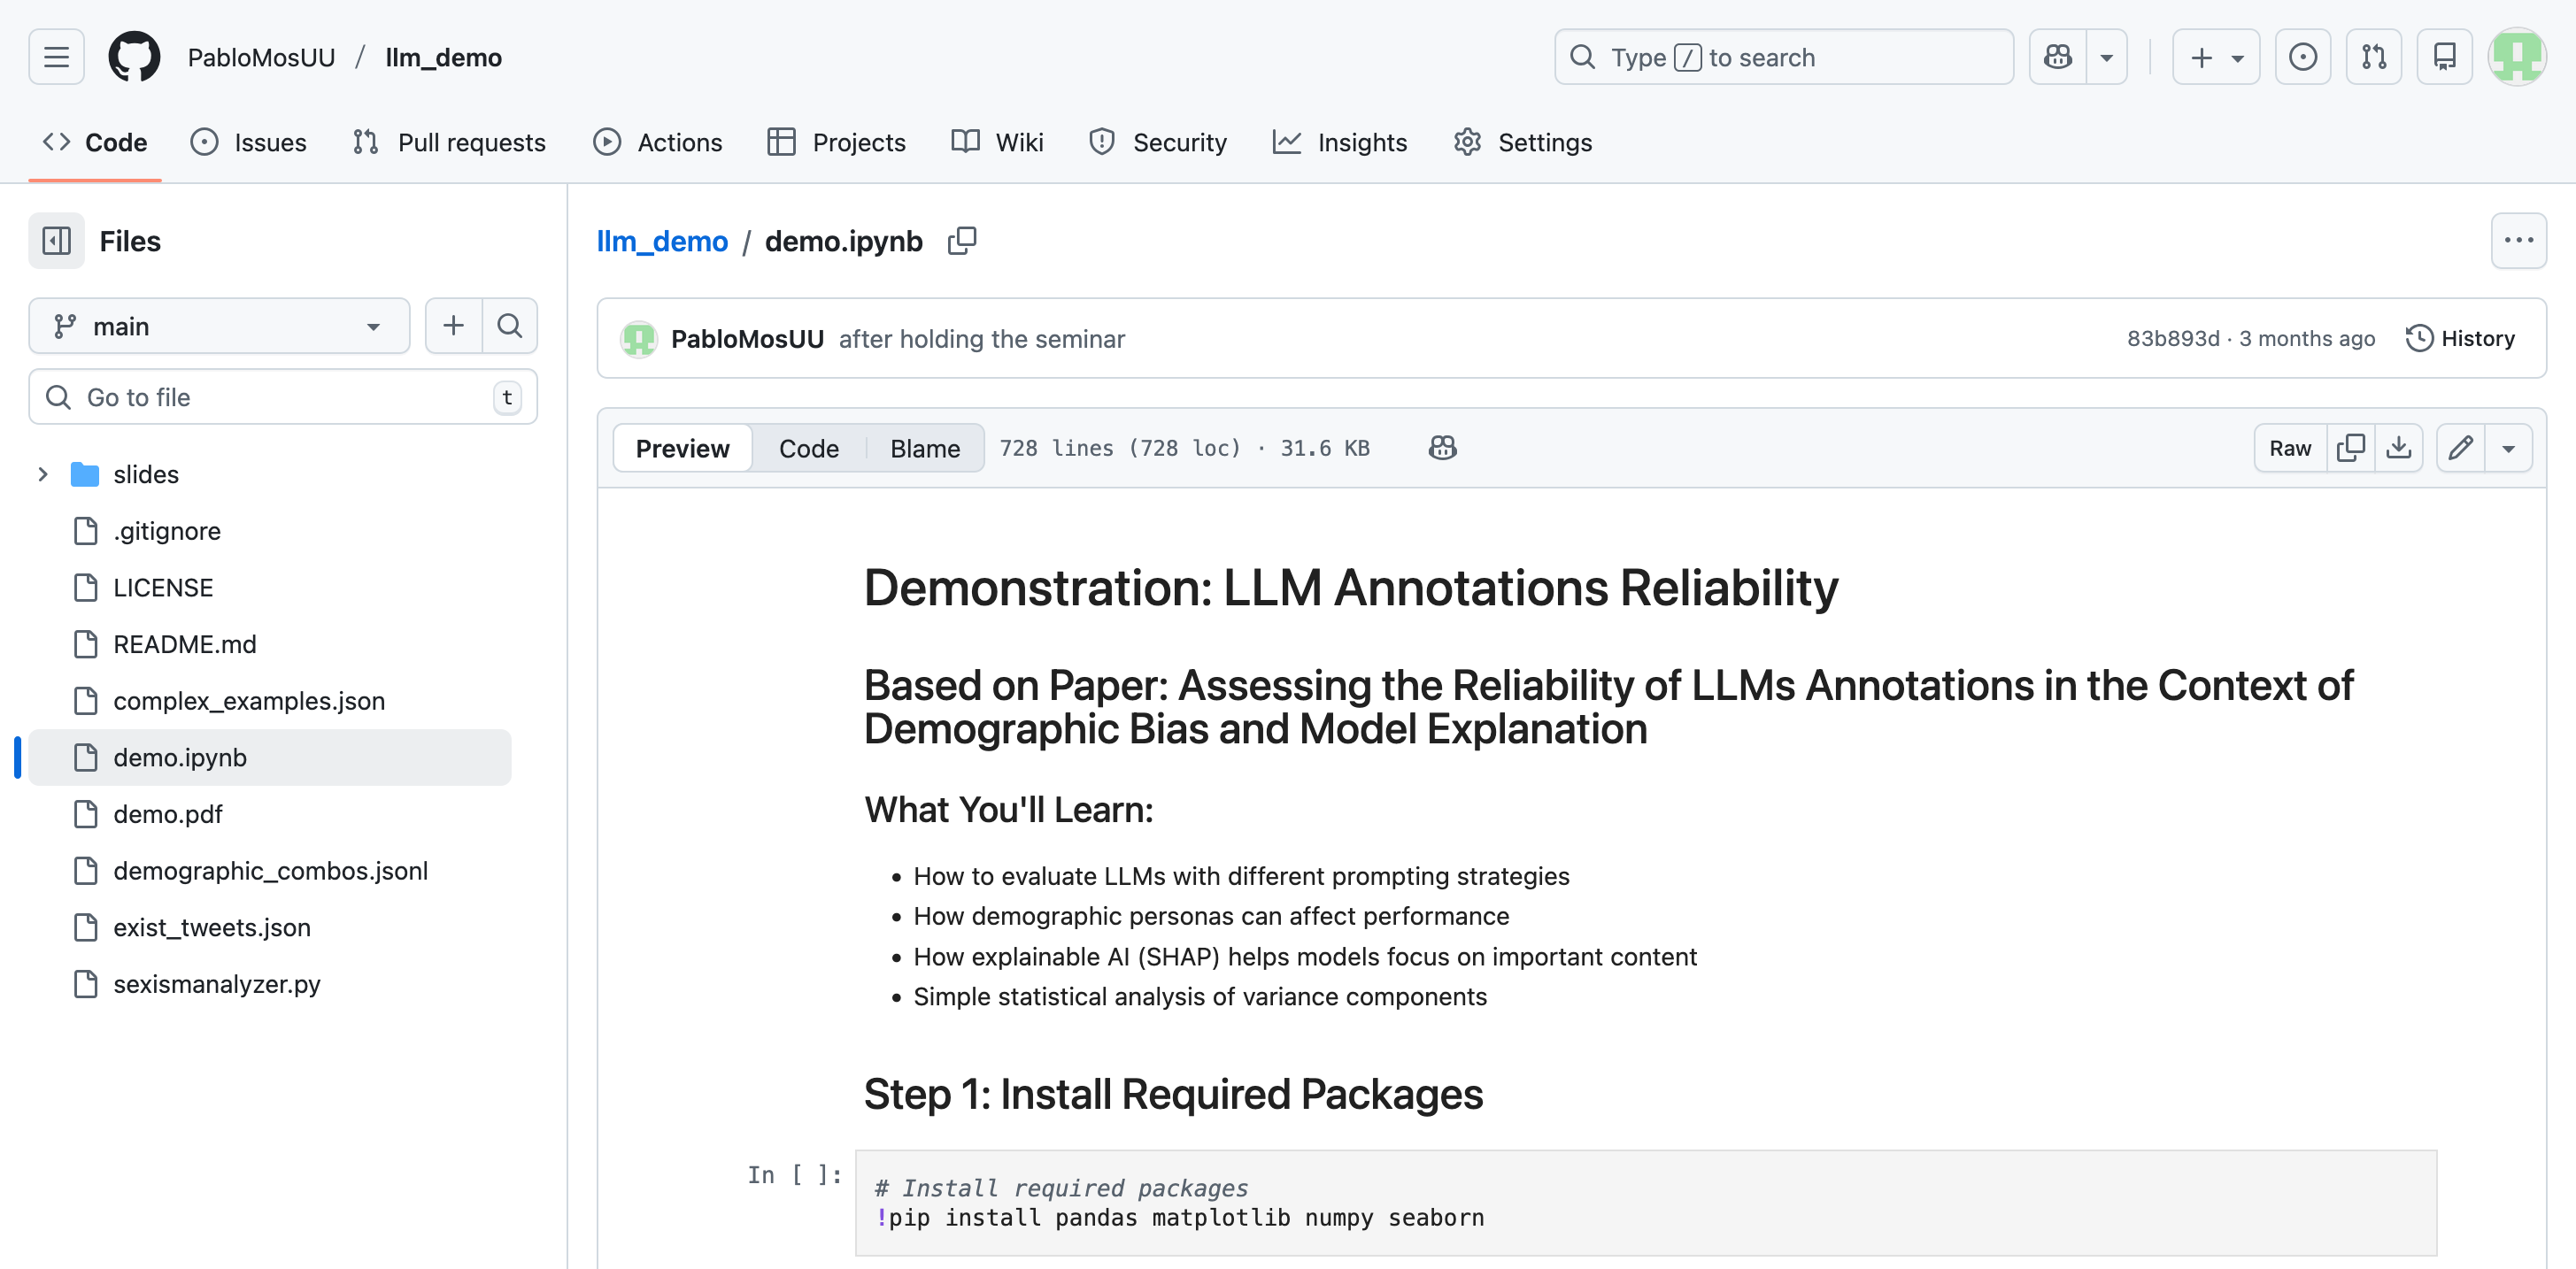
\includegraphics[width=0.8\textwidth]{img/llm_demo.png}

\footnotesize{\url{https://github.com/PabloMosUU/llm_demo}}
\end{frame}

\section{Conclusion}

\begin{frame}{Activity: Complete the Workflow Diagram}
    \textbf{Instructions}: Fill in the missing parts of this LLM research workflow
    
    \begin{center}
    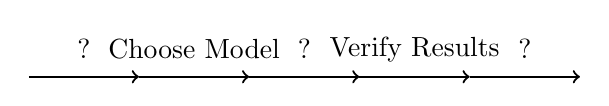
\begin{tikzpicture}[scale=0.7]
        % Incomplete diagram - students complete
        \draw[->, thick] (0,0) -- (2,0);
        \node at (1,0.5) {?};
        
        \draw[->, thick] (2,0) -- (4,0);
        \node at (3,0.5) {Choose Model};
        
        \draw[->, thick] (4,0) -- (6,0);
        \node at (5,0.5) {?};
        
        \draw[->, thick] (6,0) -- (8,0);
        \node at (7,0.5) {Verify Results};
        
        \draw[->, thick] (8,0) -- (10,0);
        \node at (9,0.5) {?};
    \end{tikzpicture}
    \end{center}
    
    \textbf{Discussion}: What steps are missing? How would you complete this?
\end{frame}

\begin{frame}{Key Takeaways: LLM Workflow}
    \begin{center}
    \smartdiagramset{set color list={blue!50,green!50,red!50,yellow!50,orange!50}}
    \smartdiagram[flow diagram:horizontal]{
        Understand LLMs,
        Choose Ethical Models,
        Apply Responsibly,
        Verify Outputs,
        Maintain Human Oversight
    }
    \end{center}
\end{frame}

\begin{frame}{Final Thoughts}
    \textbf{Remember:}
    \begin{itemize}
        \item LLMs are powerful tools, not replacements for human expertise
        \item Always prioritize ethics, privacy, and transparency
        \item Verify outputs and maintain critical thinking
    \end{itemize}
    
    \vfill
    \centering
    \textbf{Happy researching with AI!}
\end{frame}

\end{document}